% !TeX program = xelatex
\documentclass[aspectratio=169]{beamer}
\usepackage{booktabs}
\usetheme{metropolis}           % Use metropolis theme
\title[Ideal Splitter Optimization]{Lecture IV: Optimizing Ideal Splitters}
\subtitle{Making ideal splitters practical for use in the real world}
\date{}
\author{\textbf{Instructor:} Andrews54757}
\institute{
    CSE269: Introduction to Encoded Storage\\
    S$\infty$ntech Annals
}
\logo{
\includegraphics[height=0.7cm]{logo3.png}}
\begin{document}
\maketitle

\begin{frame}
\frametitle{Overview}
\tableofcontents
\end{frame}

\section{1. Optimizing the Loaders}

\subsection{1.1 Basic Optimizations}

\begin{frame}
	\frametitle{1.1 Basic Loader Optimizations}
    

	\begin{figure}
        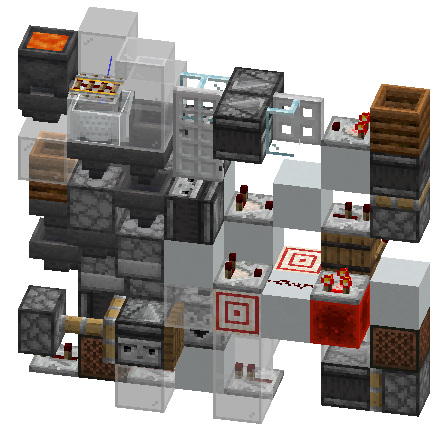
\includegraphics[width=0.3\textwidth]{oldloader.png}
		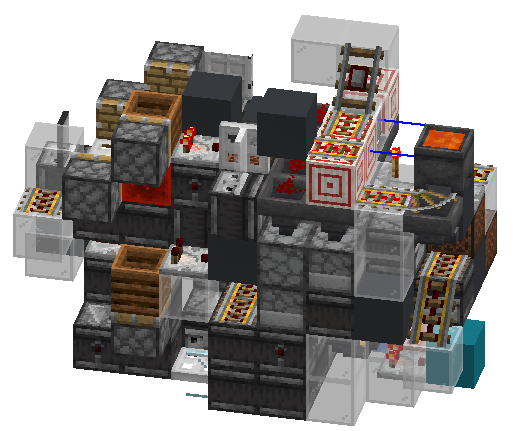
\includegraphics[width=0.35\textwidth]{newloader.png}
		\caption{Old 4x loader (left) vs new 8x loader (right)}
	\end{figure}


    \begin{itemize}
		\item Twice as fast so half the latency
		\item Less hoppers per hopperspeed (3 vs 1.38)
		\item Less loaders = simpler logic
	\end{itemize}
	
\end{frame}

\begin{frame}
	\frametitle{1.1 Basic Loader Optimizations Contd.}
    \begin{columns}
        \column{0.4\linewidth}

	\begin{figure}
		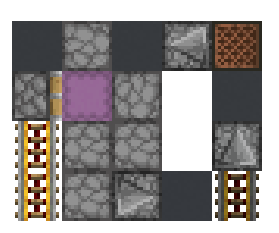
\includegraphics[width=1\textwidth]{toploaderview.png}
		\caption{Loader layout}
	\end{figure}

    \column{0.6\linewidth}
    \begin{itemize}
        \item Simple loader layout
		\item No comparator readouts
		\item \textbf{How does it know when to break the box?}
		\item A: Break box when the task ends
	\end{itemize}
    \end{columns}
	
\end{frame}


\begin{frame}
	\frametitle{1.1 Terminology: What is a task?}
    
    Work to be done by the loader. In this case, a task is a set of items that need to be loaded into a box.
    \begin{itemize}
        \item Each task has only one item type
        \item Each task fits inside one box ($\leq 27$ stacks)
        \begin{itemize}
            \item Exception for last task of a type, $< 28$ stacks (come back to it later)
        \end{itemize}
        \item It takes time to finish a task because it needs to load items into a box. ($O(n)$ where n is the number of items in the task)
    \end{itemize}
	
\end{frame}

\begin{frame}
	\frametitle{1.1 Terminology: What is a task?}
    
\includegraphics[width=1\textwidth]{tasks.png}
    \break
    In terms of implementation, a task is a collection of minecarts where.
    \begin{itemize}
        \item Each minecart preferrably contains one full stack
        \item A new task begins whenever 27 carts are counted, or when the item type changes.
        \item We recieve a redstone signal when a new task begins
    \end{itemize}

\end{frame}
\subsection{1.2 Queueing}

\begin{frame}
	\frametitle{1.2 Queueing Tasks}
    \begin{itemize}
        \item The ideal splitter outputs tasks at $\sim$32x hopperspeed.
        \item Each box loader can only consume tasks at 8x hopperspeed.
        \item Splitter is 4x faster than the loader, so need 4 loaders
        \item Task size varies, so need to queue tasks to efficiently distribute work
        \item \textbf{What happens if we don't queue tasks?}

    \end{itemize}

    
\end{frame}


\begin{frame}
	\frametitle{1.2 Not Queueing Tasks}

    Imagine we have 27 stacks of dirt, a stack of redstone, a stack of emeralds, a stack of glowstone, and a stack of diamonds.

    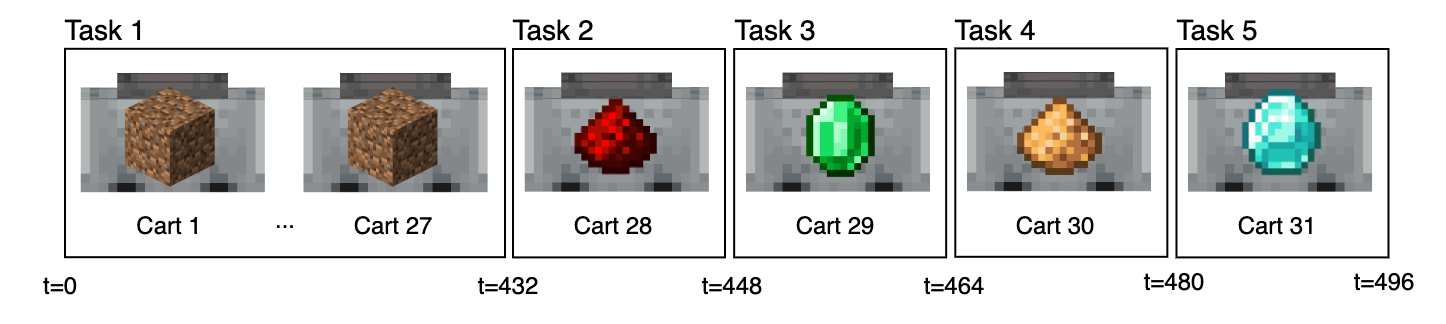
\includegraphics[width=1\textwidth]{example1.png}

    Each task is assigned to a loader that is not busy with another task.
\end{frame}

\begin{frame}
	\frametitle{1.2 Not Queueing Tasks}
    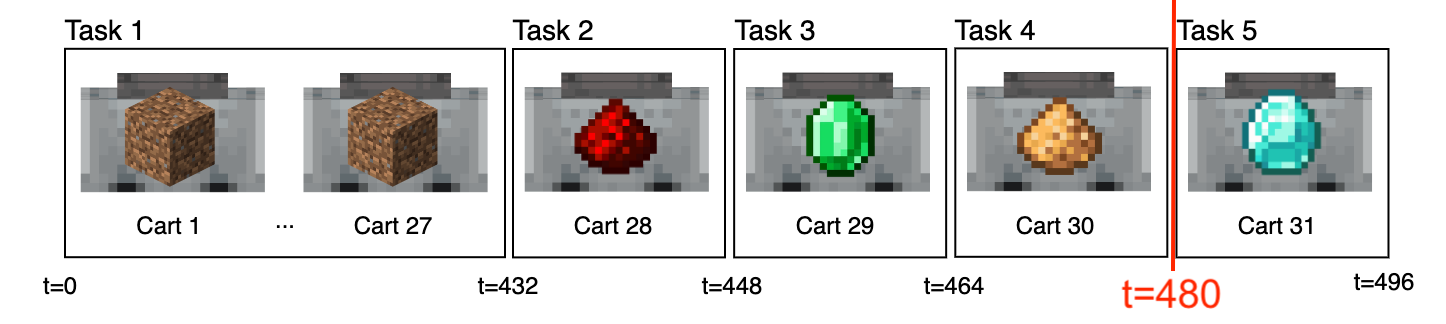
\includegraphics[width=1\textwidth]{example1.1.png}
    \begin{columns}
        \column{0.3\linewidth}

    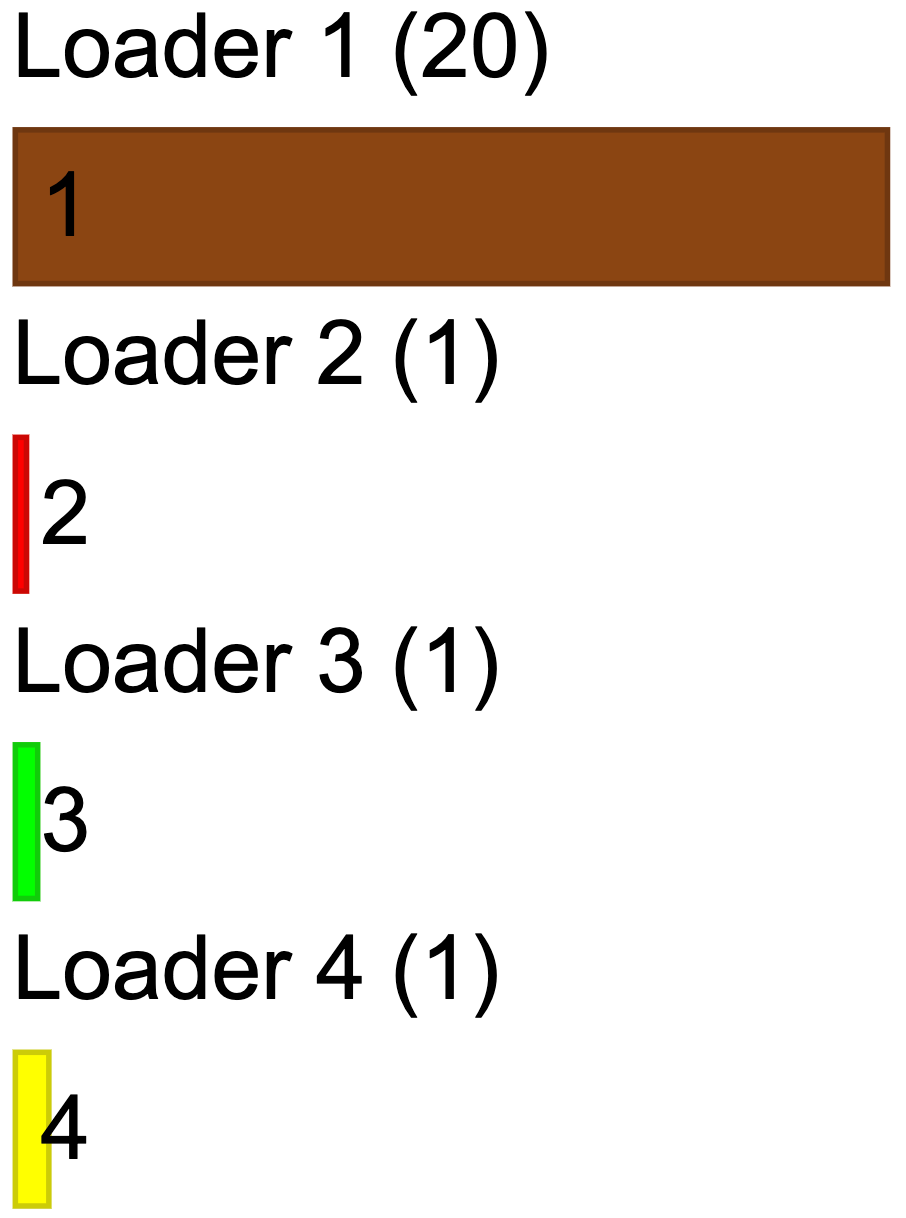
\includegraphics[height=4.5cm]{example1result.png}

        \column{0.7\linewidth}
        \textbf{Where does the diamond go?}

        - Old design: Add more loaders!

        - Hence 30 4x loaders

        - $30x4 > 32$: super wasteful

    \end{columns}

\end{frame}


\begin{frame}
	\frametitle{1.2 Queueing Tasks}
    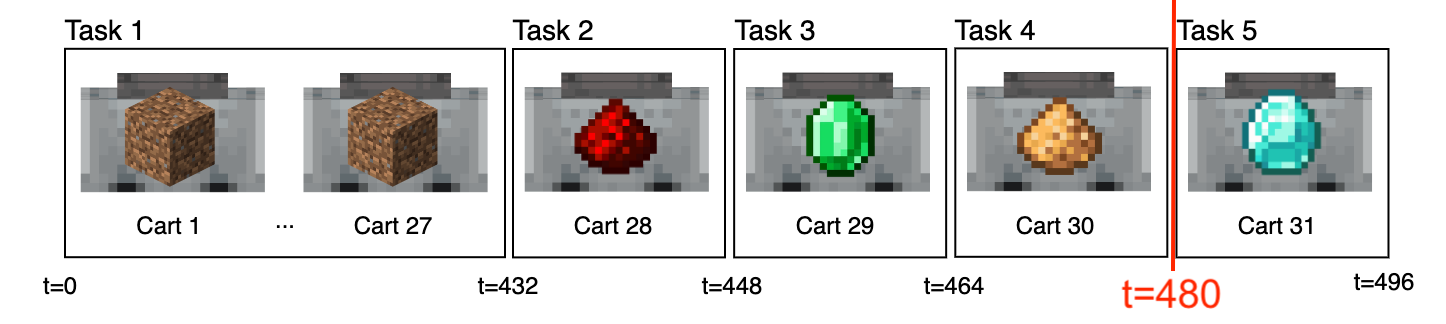
\includegraphics[width=1\textwidth]{example1.1.png}
    \begin{columns}
        \column{0.3\linewidth}
    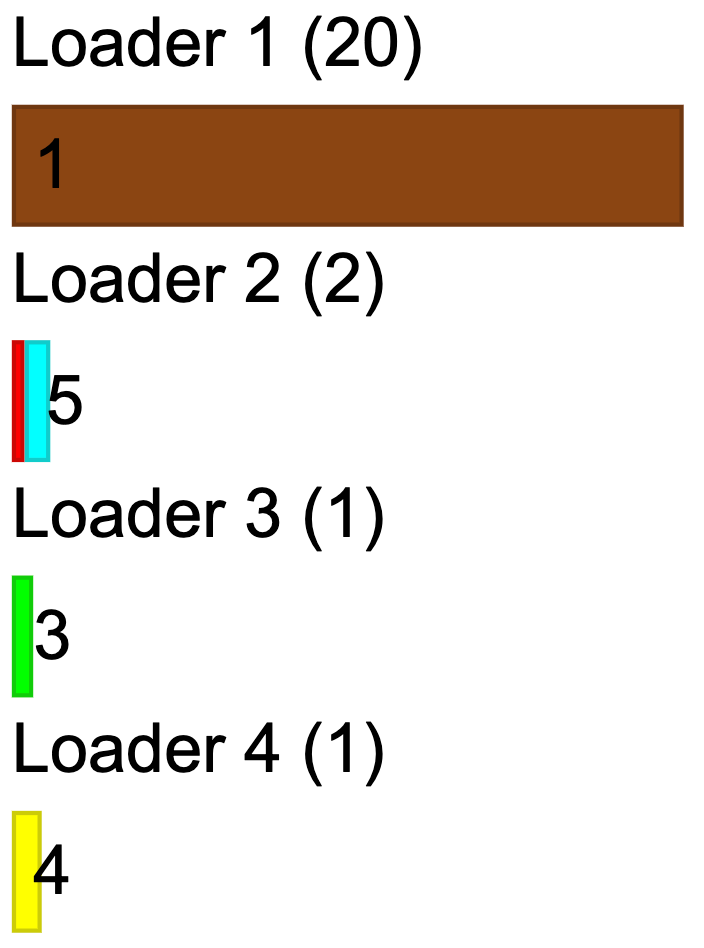
\includegraphics[height=4.5cm]{example1result2.png}

        \column{0.7\linewidth}
        \textbf{Queueing tasks}

        - Add diamond task to loader 2's queue

        - Loader 2 will load the diamond task after it finishes the redstone task

        - Don't need more loaders!

    \end{columns}

\end{frame}


\begin{frame}
	\frametitle{1.2 Queueing Tasks}
    \begin{columns}
        \column{0.4\linewidth}

	\begin{figure}
		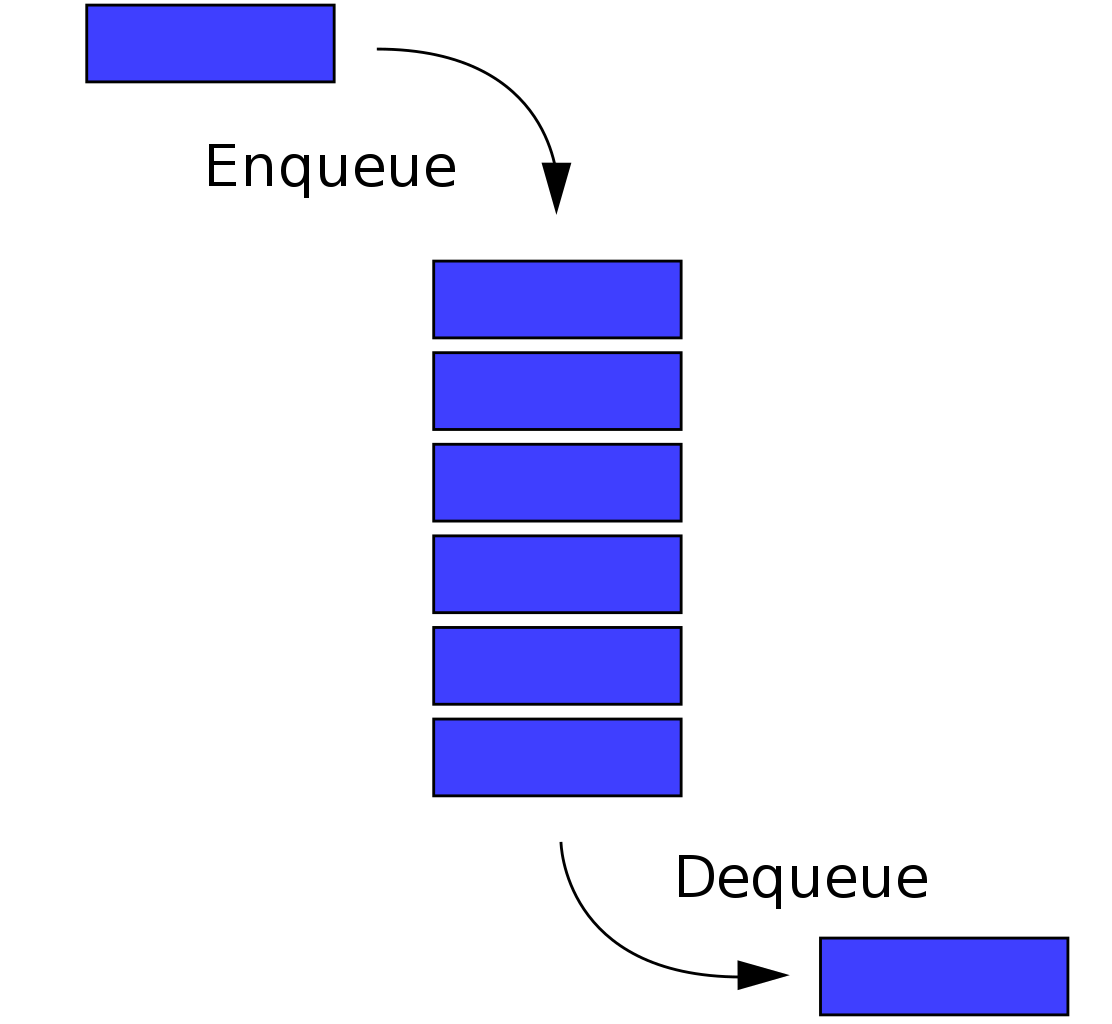
\includegraphics[width=1\textwidth]{fifo.png}
		\caption{FIFO queue}
	\end{figure}

    \column{0.6\linewidth}
    \begin{itemize}
        \item A FIFO queue stores items in a line
		\item Items are added to the back and removed from the front
		\item Order preserving, first in first out (FIFO)
		\item \textbf{How can we make a FIFO queue in minecraft?}
		\item A: Stacked minecarts
	\end{itemize}
    \end{columns}
\end{frame}

\subsection{1.3 Load Balancing}
\begin{frame}
	\frametitle{1.3 Load Balancing Reduces Latency}
    
    Latency is the amount of time it takes for a task to begin processing. Proper load balancing reduces the latency by distributing tasks evenly across loaders.

    \begin{columns}
        \column{0.5\linewidth}
        \centering
        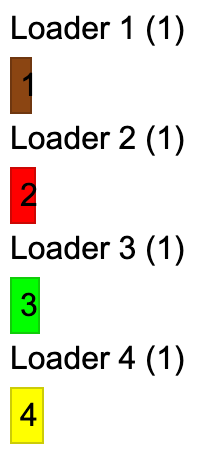
\includegraphics[height=5cm]{latencygood.png}

        \textcolor{green}{Low latency}

        \column{0.5\linewidth}
        \centering
        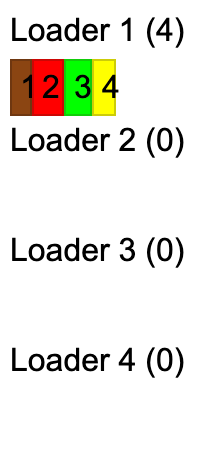
\includegraphics[height=5cm]{latencybad.png}

        \textcolor{red}{High latency}
    \end{columns}
\end{frame}

\begin{frame}
	\frametitle{1.3 Ideal Load Balancing}
    
    The ideal solution for this online load balancing problem is to distribute tasks to the least-busy loader. (similar to least connections algorithm)

    The problem is that we need to compare the queue sizes with each loader in order to determine the least busy loader.

    This is too complicated to do in Minecraft pragmatically.
\end{frame}

\begin{frame}
    \frametitle{1.3 Good Enough Load Balancing}

    \textbf{Simple isEmpty Balancing Algorithm}

    \begin{itemize}
        \item If an empty loader is available, assign the task to the empty loader
        \item Otherwise, assign the task to any loader with $< 21$ carts in its queue
    \end{itemize}

    Easily implemented with comparator logic
    \begin{figure}
        \centering
        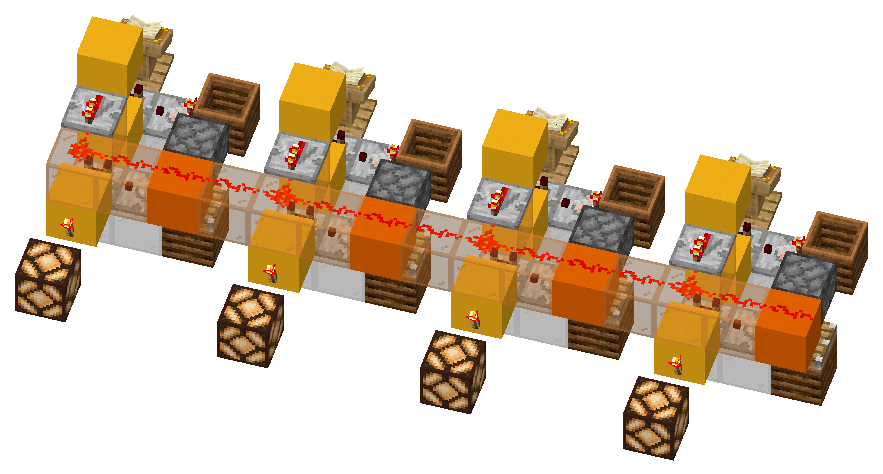
\includegraphics[width=0.5\textwidth]{simple.png}
		\caption{Simple isEmpty balancing circuit}
	\end{figure}
  

\end{frame}

\begin{frame}
    \frametitle{1.3 Good Enough Load Balancing}

    \textbf{Weighted isEmpty Balancing Algorithm}

    \begin{itemize}
        \item Threshold for first 50\% of loaders is 11 carts instead of 21
        \item Gives more chances for further loaders to be used
    \end{itemize}

    \begin{figure}
        \centering
        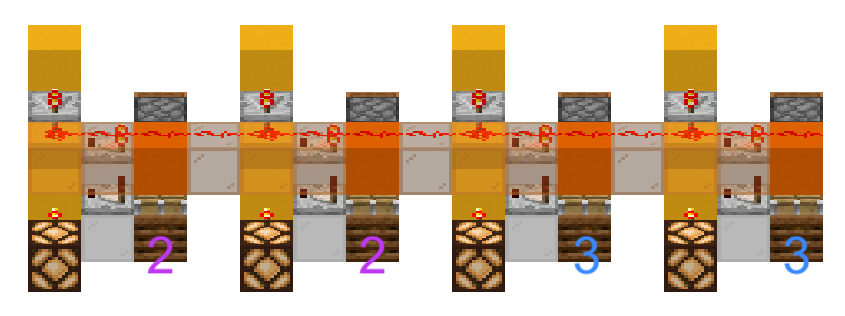
\includegraphics[width=0.8\textwidth]{weighted.png}
		\caption{Weighted isEmpty balancing circuit}
	\end{figure}

\end{frame}

\begin{frame}
    \frametitle{1.3 Good Enough Load Balancing}

    \begin{table}
        \begin{tabular}{l l l}
            \toprule
            \textbf{Algorithm} & \textbf{Difficulty} & \textbf{Average Latency (s)}\\
            \midrule
            Ideal & Hard & 5.27 \\
            Weighted isEmpty balancing & OK & 11.59 \\
            Simple isEmpty balancing & OK & 26.84 \\
            No balancing & Easy & 42.14 \\
            \bottomrule
        \end{tabular}
        \caption{Load balancing algorithms compared}
    \end{table}

    Relative to the no balancing algorithm, the weighted isEmpty balancing algorithm is 83\% as good as the ideal algorithm, but much easier to implement.
\end{frame}

\section{2. Optimizing the Cart Splitter}
\subsection{2.1 Item Entity Merging Problem}

\begin{frame}
    \frametitle{2.1 Item Entities are Laggy}
    \begin{itemize}
        \item Most ($>50\%$) of the machine's lag is caused by item entities
        \item Item entity merging is particularly laggy
    \end{itemize}

    \begin{figure}
        \centering
        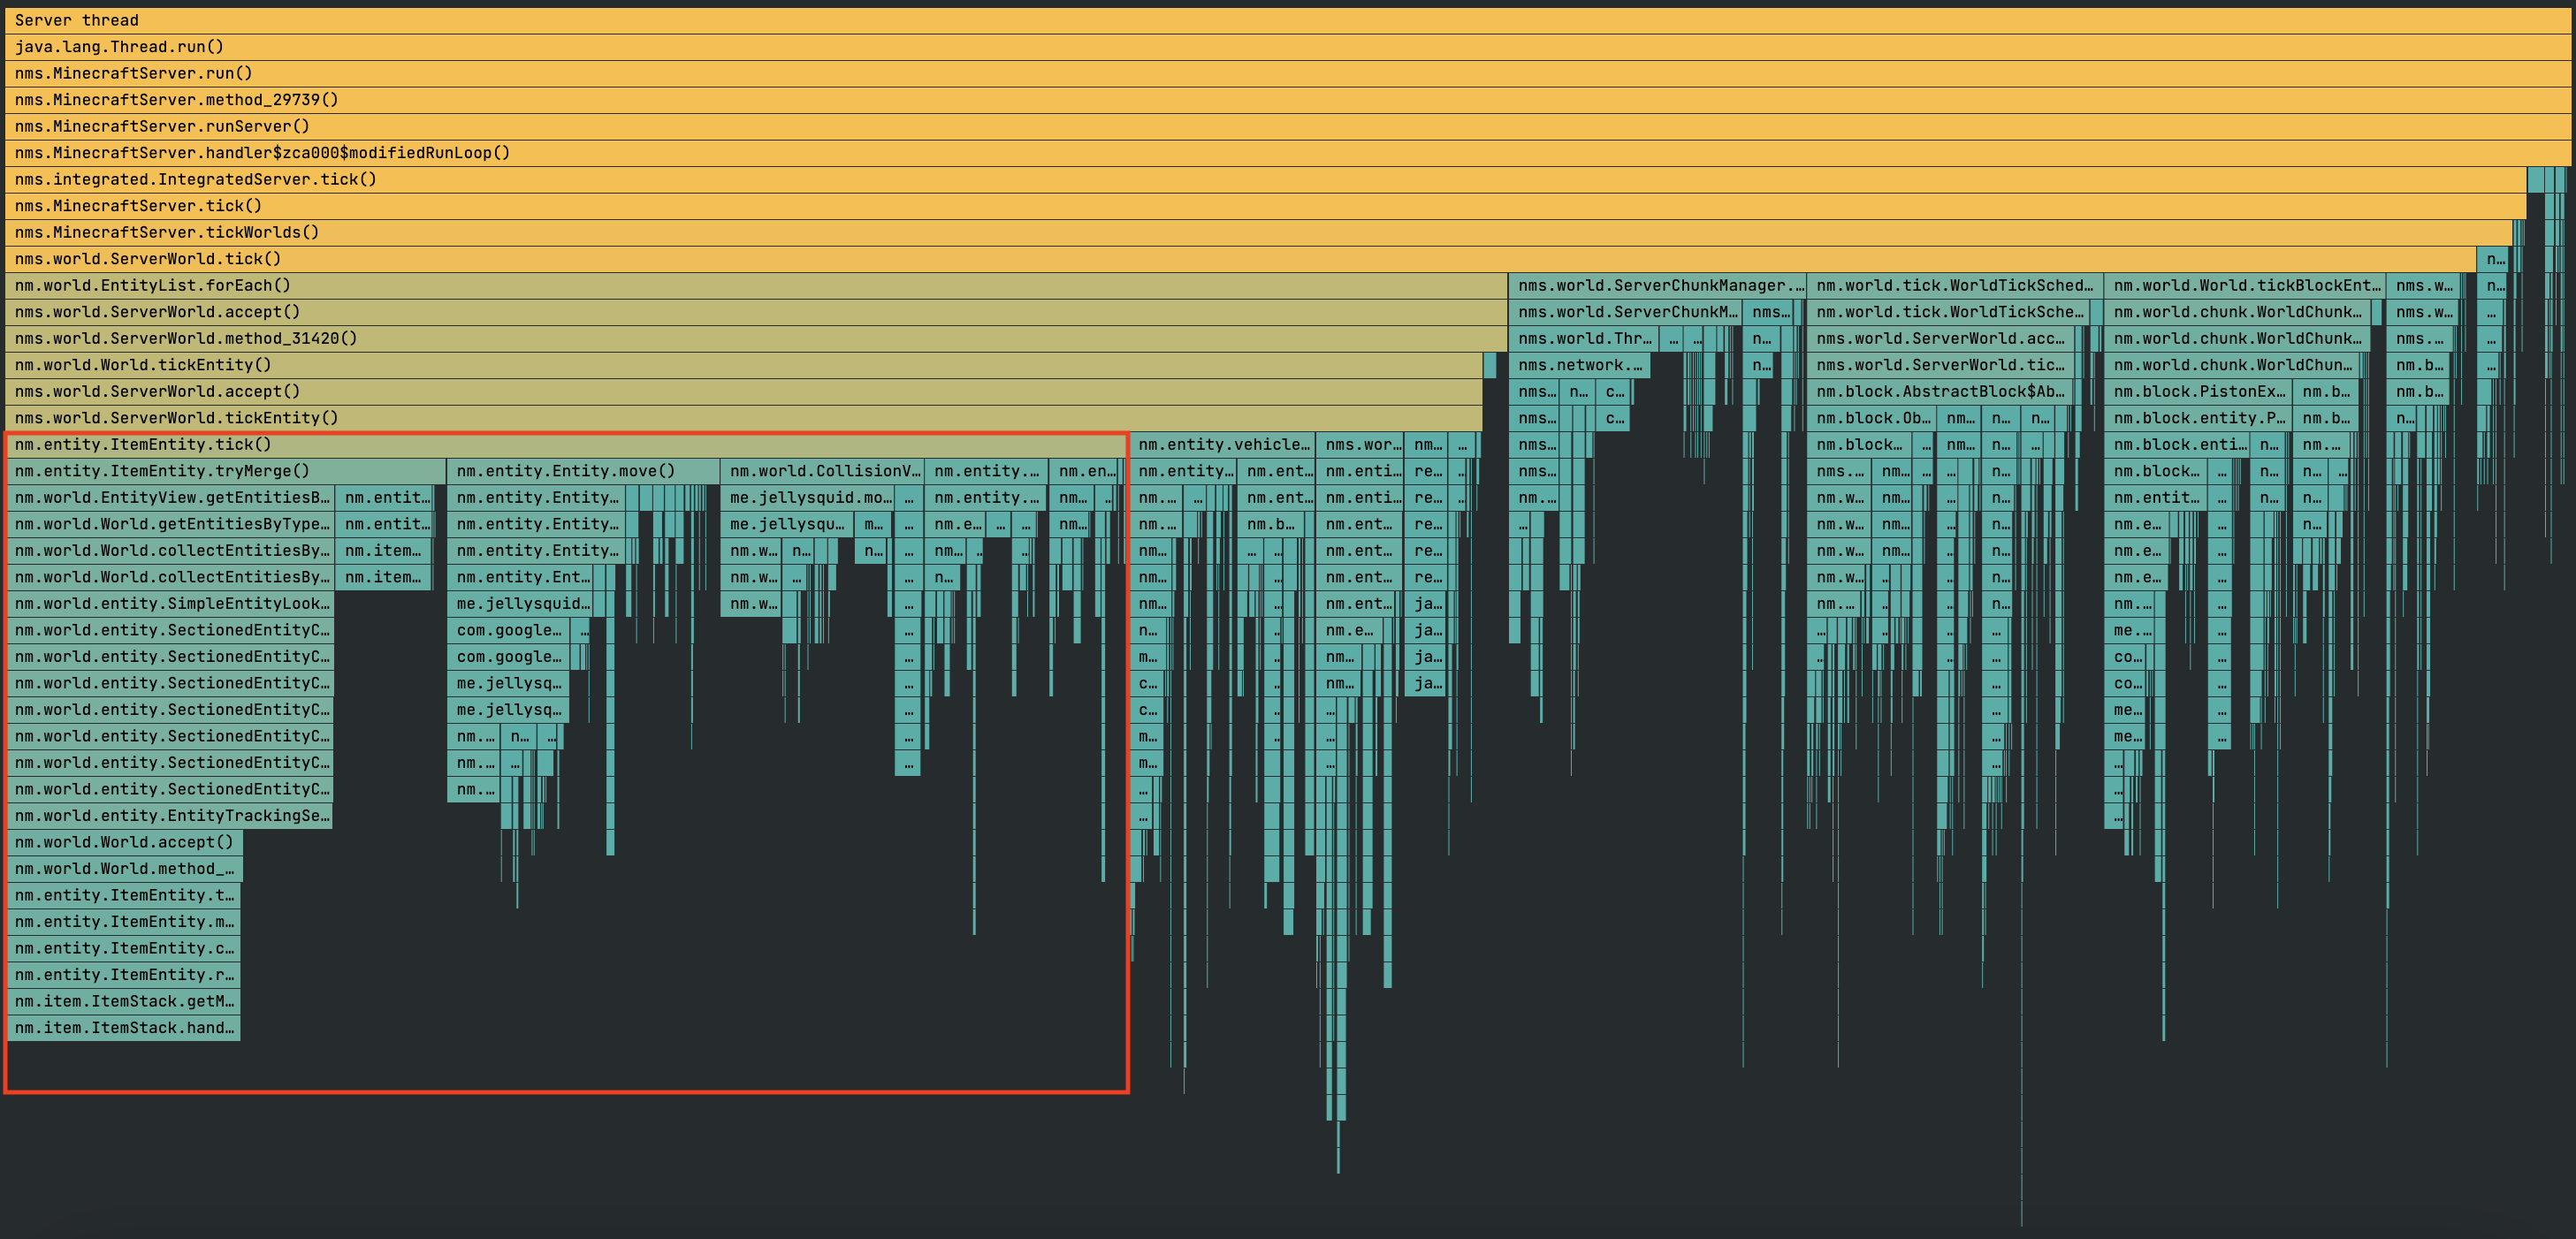
\includegraphics[width=0.7\textwidth]{itemlag.png}
        \caption{V1 Ideal Splitter during first minute of operation with Mumbo's Hermitcraft items (62k items, 1200+ item entities)}
    \end{figure}
\end{frame}


\begin{frame}
    \frametitle{2.1 Item Entity Merging Problem}
    \begin{itemize}
        \item Item entities must be merged otherwise may additional cause partial boxes
        \item Game merges item entities up to once every 40 gt when they are still
        \item When item entities are moving, they are merged up to once every 2gt
    \end{itemize}

    \begin{figure}
        \centering
        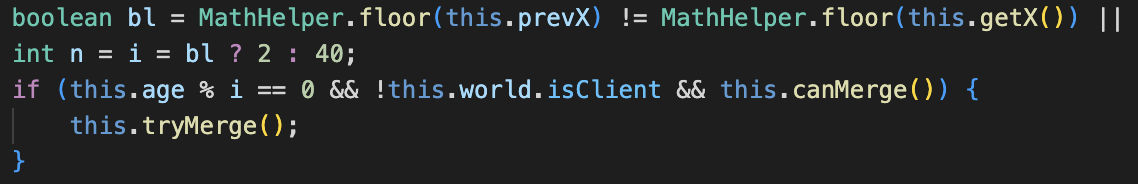
\includegraphics[width=0.93\textwidth]{mergecode.png}
        \caption{Item entity merging code}
    \end{figure}
    
\end{frame}

\begin{frame}
    \frametitle{2.1 Item Entity Merging Problem}
    \begin{itemize}
        \item Old solution: Bounce item entities between slime blocks to keep them moving and force them to merge
        \begin{itemize}
            \item Works, but is very laggy
        \end{itemize}
    \end{itemize}

    \begin{figure}
        \centering
        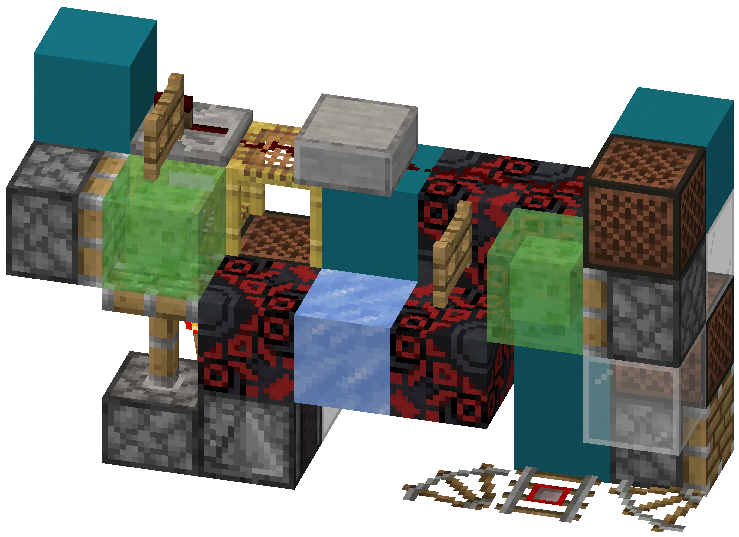
\includegraphics[width=0.45\textwidth]{bouncer.png}
        \caption{Item entity bouncer}
    \end{figure}
\end{frame}


\begin{frame}
    \frametitle{2.1 Item Entity Merging Problem}
    \textbf{How can we ensure that item entities merge without bouncing them?}
    
    A: Keep carts under the item entities longer so that 40gt merge interval is sufficient

    \centering
    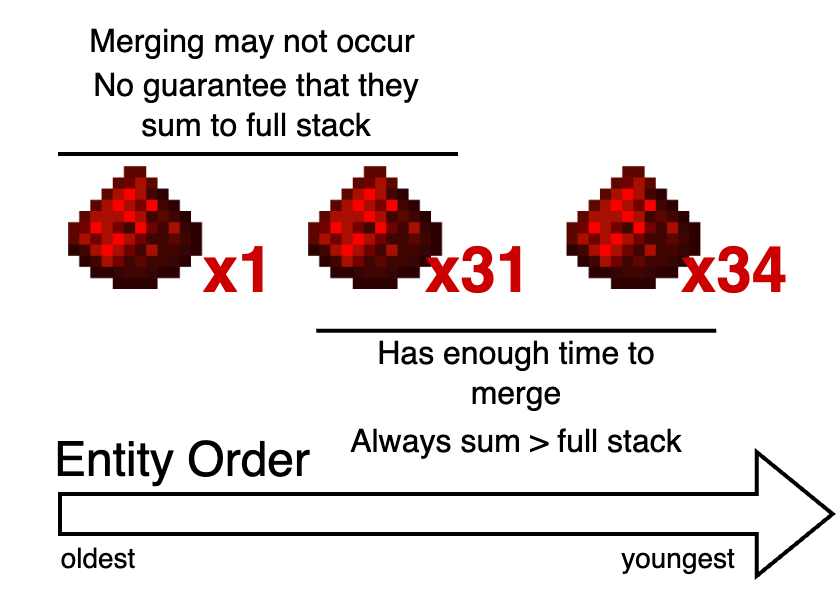
\includegraphics[width=0.4\textwidth]{mergelogic2.png}

    If cart is under for at least 3gt, full stack is guaranteed.
\end{frame}


\begin{frame}
    \frametitle{2.1 Item Entity Merging Problem}
    In practice, cart was already under item entities for at least 4gt. However, it wasn't being detected by the isFull comparator due to it failing to schedule an update.
    \begin{itemize}
        \item Comparator checks that its value can change before scheduling an update to change it 2gt later
        \item Ensure comparator always schedules by disabling side-subtract for 2gt pulse
    \end{itemize}

    \centering
    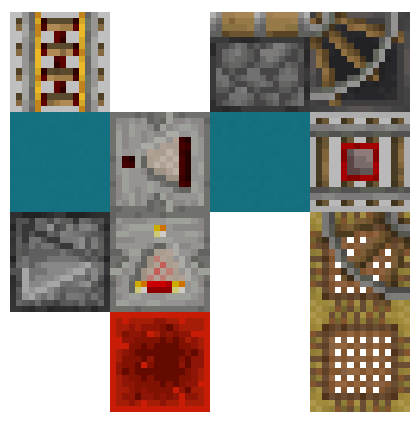
\includegraphics[width=0.3\textwidth]{comptrick.png}
\end{frame}


\subsection{2.2 Cart-based Unloader}
\begin{frame}
    \frametitle{2.2 Cart-based Unloader and Item Refresher}
    \begin{columns}
        \column{0.5\linewidth}

	\begin{figure}
		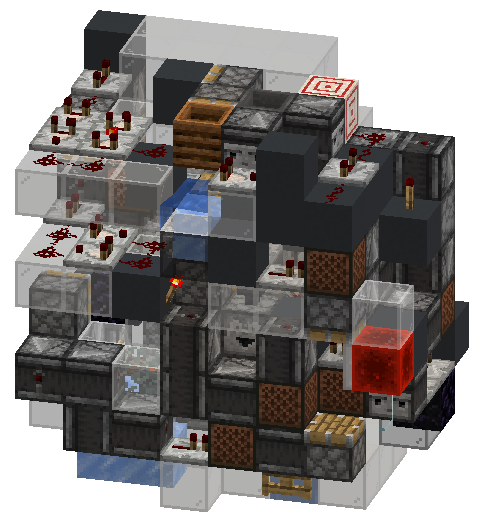
\includegraphics[width=0.8\textwidth]{cartyeeter.png}
		\caption{Cart-based Unloader}
	\end{figure}

    \column{0.6\linewidth}
    \begin{itemize}
        \item Box yeeting wastes boxes
        \item Dolphin AI causes static lag
        \item \textbf{Solution:} Use carts to unload boxes and refresh item entity age
        \begin{itemize}
            \item But is much larger and a little slower than box yeeter and dolphin
            \item Not recommended for anybody except STD-purists
        \end{itemize}
	\end{itemize}
    \end{columns}
\end{frame}

\section{3. Implementation}

{
\logo{}
\begin{frame}
    \frametitle{3.1 Full Diagram}
    \centering
    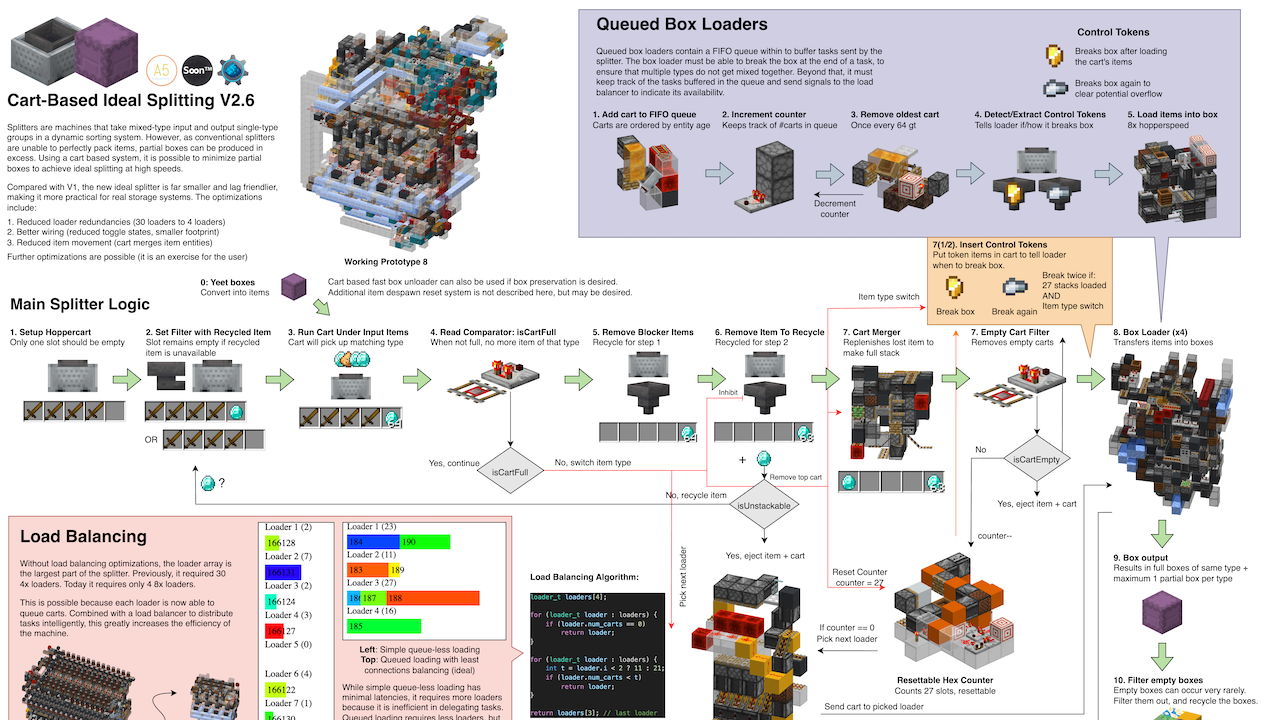
\includegraphics[width=0.75\paperwidth]{IdealSplitting3.png}
\end{frame}

\begin{frame}
    \frametitle{3.2 Control Tokens}
    \centering
    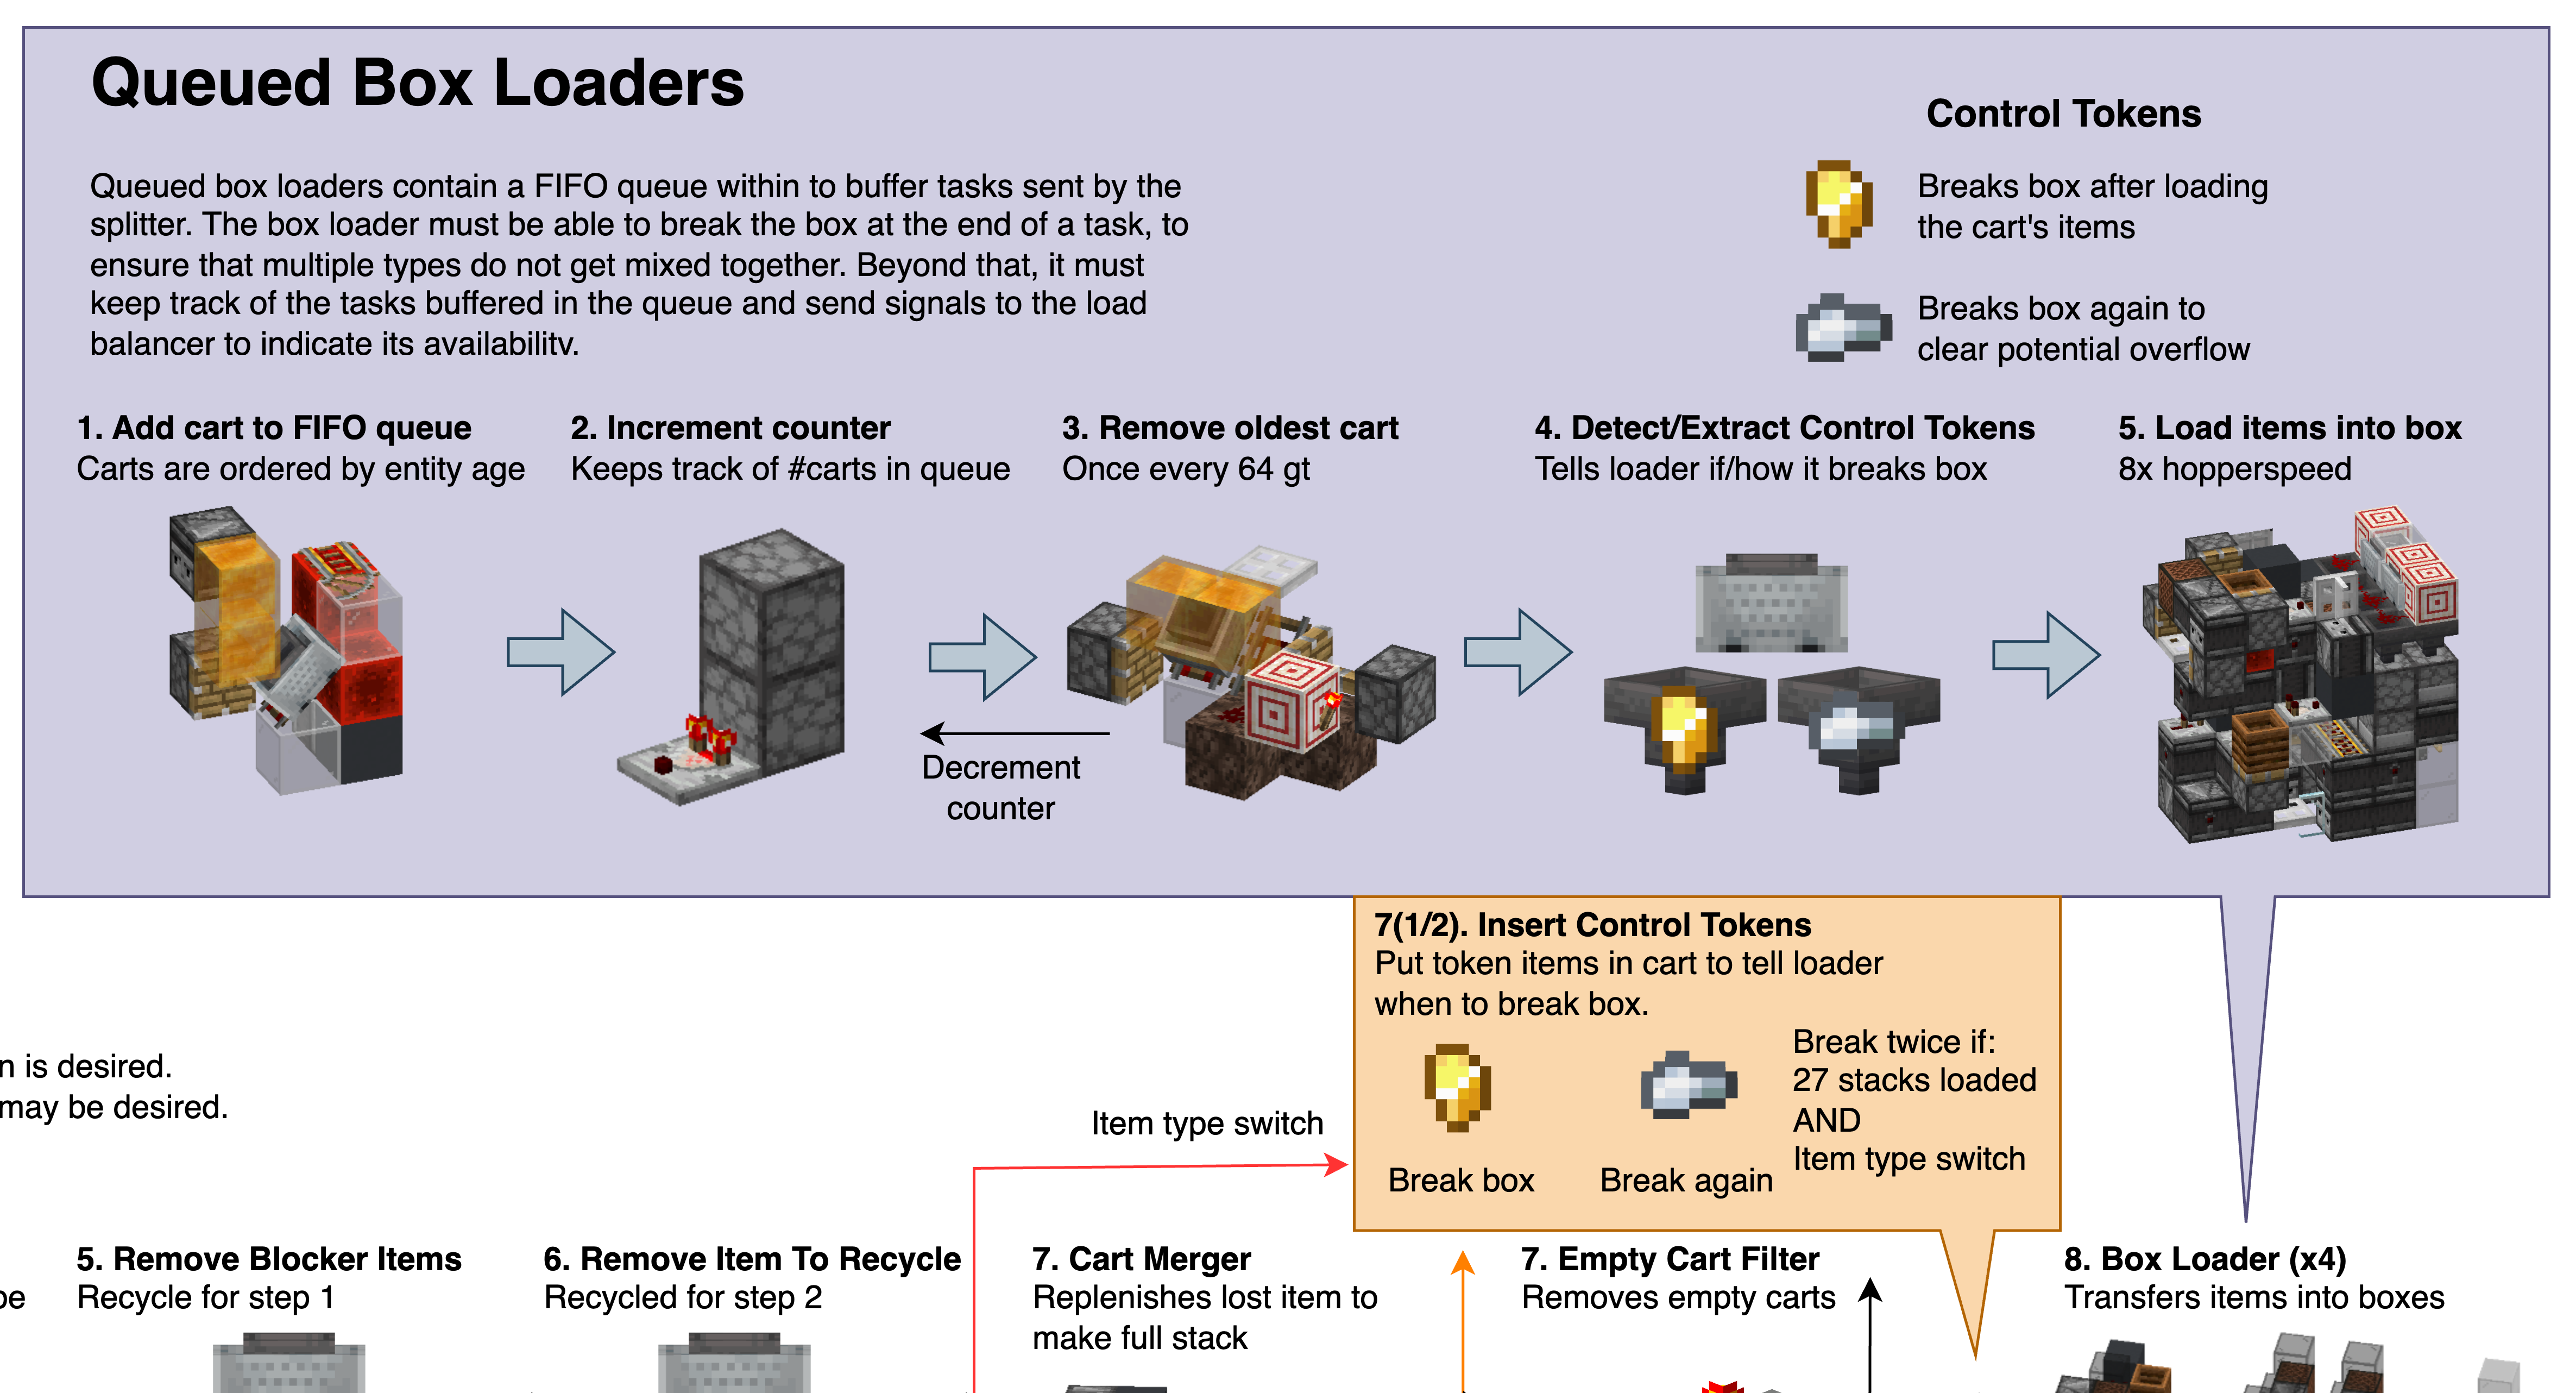
\includegraphics[width=0.85\paperwidth]{IdealSplitting3zoom.png}
\end{frame}
}

\begin{frame}
    \frametitle{3.2 Cart Merger Shenanigans}
    \begin{itemize}
        \item Cart merger buffers one cart to ensure other carts have full stack
        \item That cart is ejected whenever item type switches
        \item Cart is appended to previous task
        \item The task might have $>27$ stacks (but still $\leq28$)
        \item Need to break box \textbf{twice} if it has $>27$ stacks
    \end{itemize}

\end{frame}

{
\logo{}
\begin{frame}
    \frametitle{3.2 Control Tokens}
    \centering
    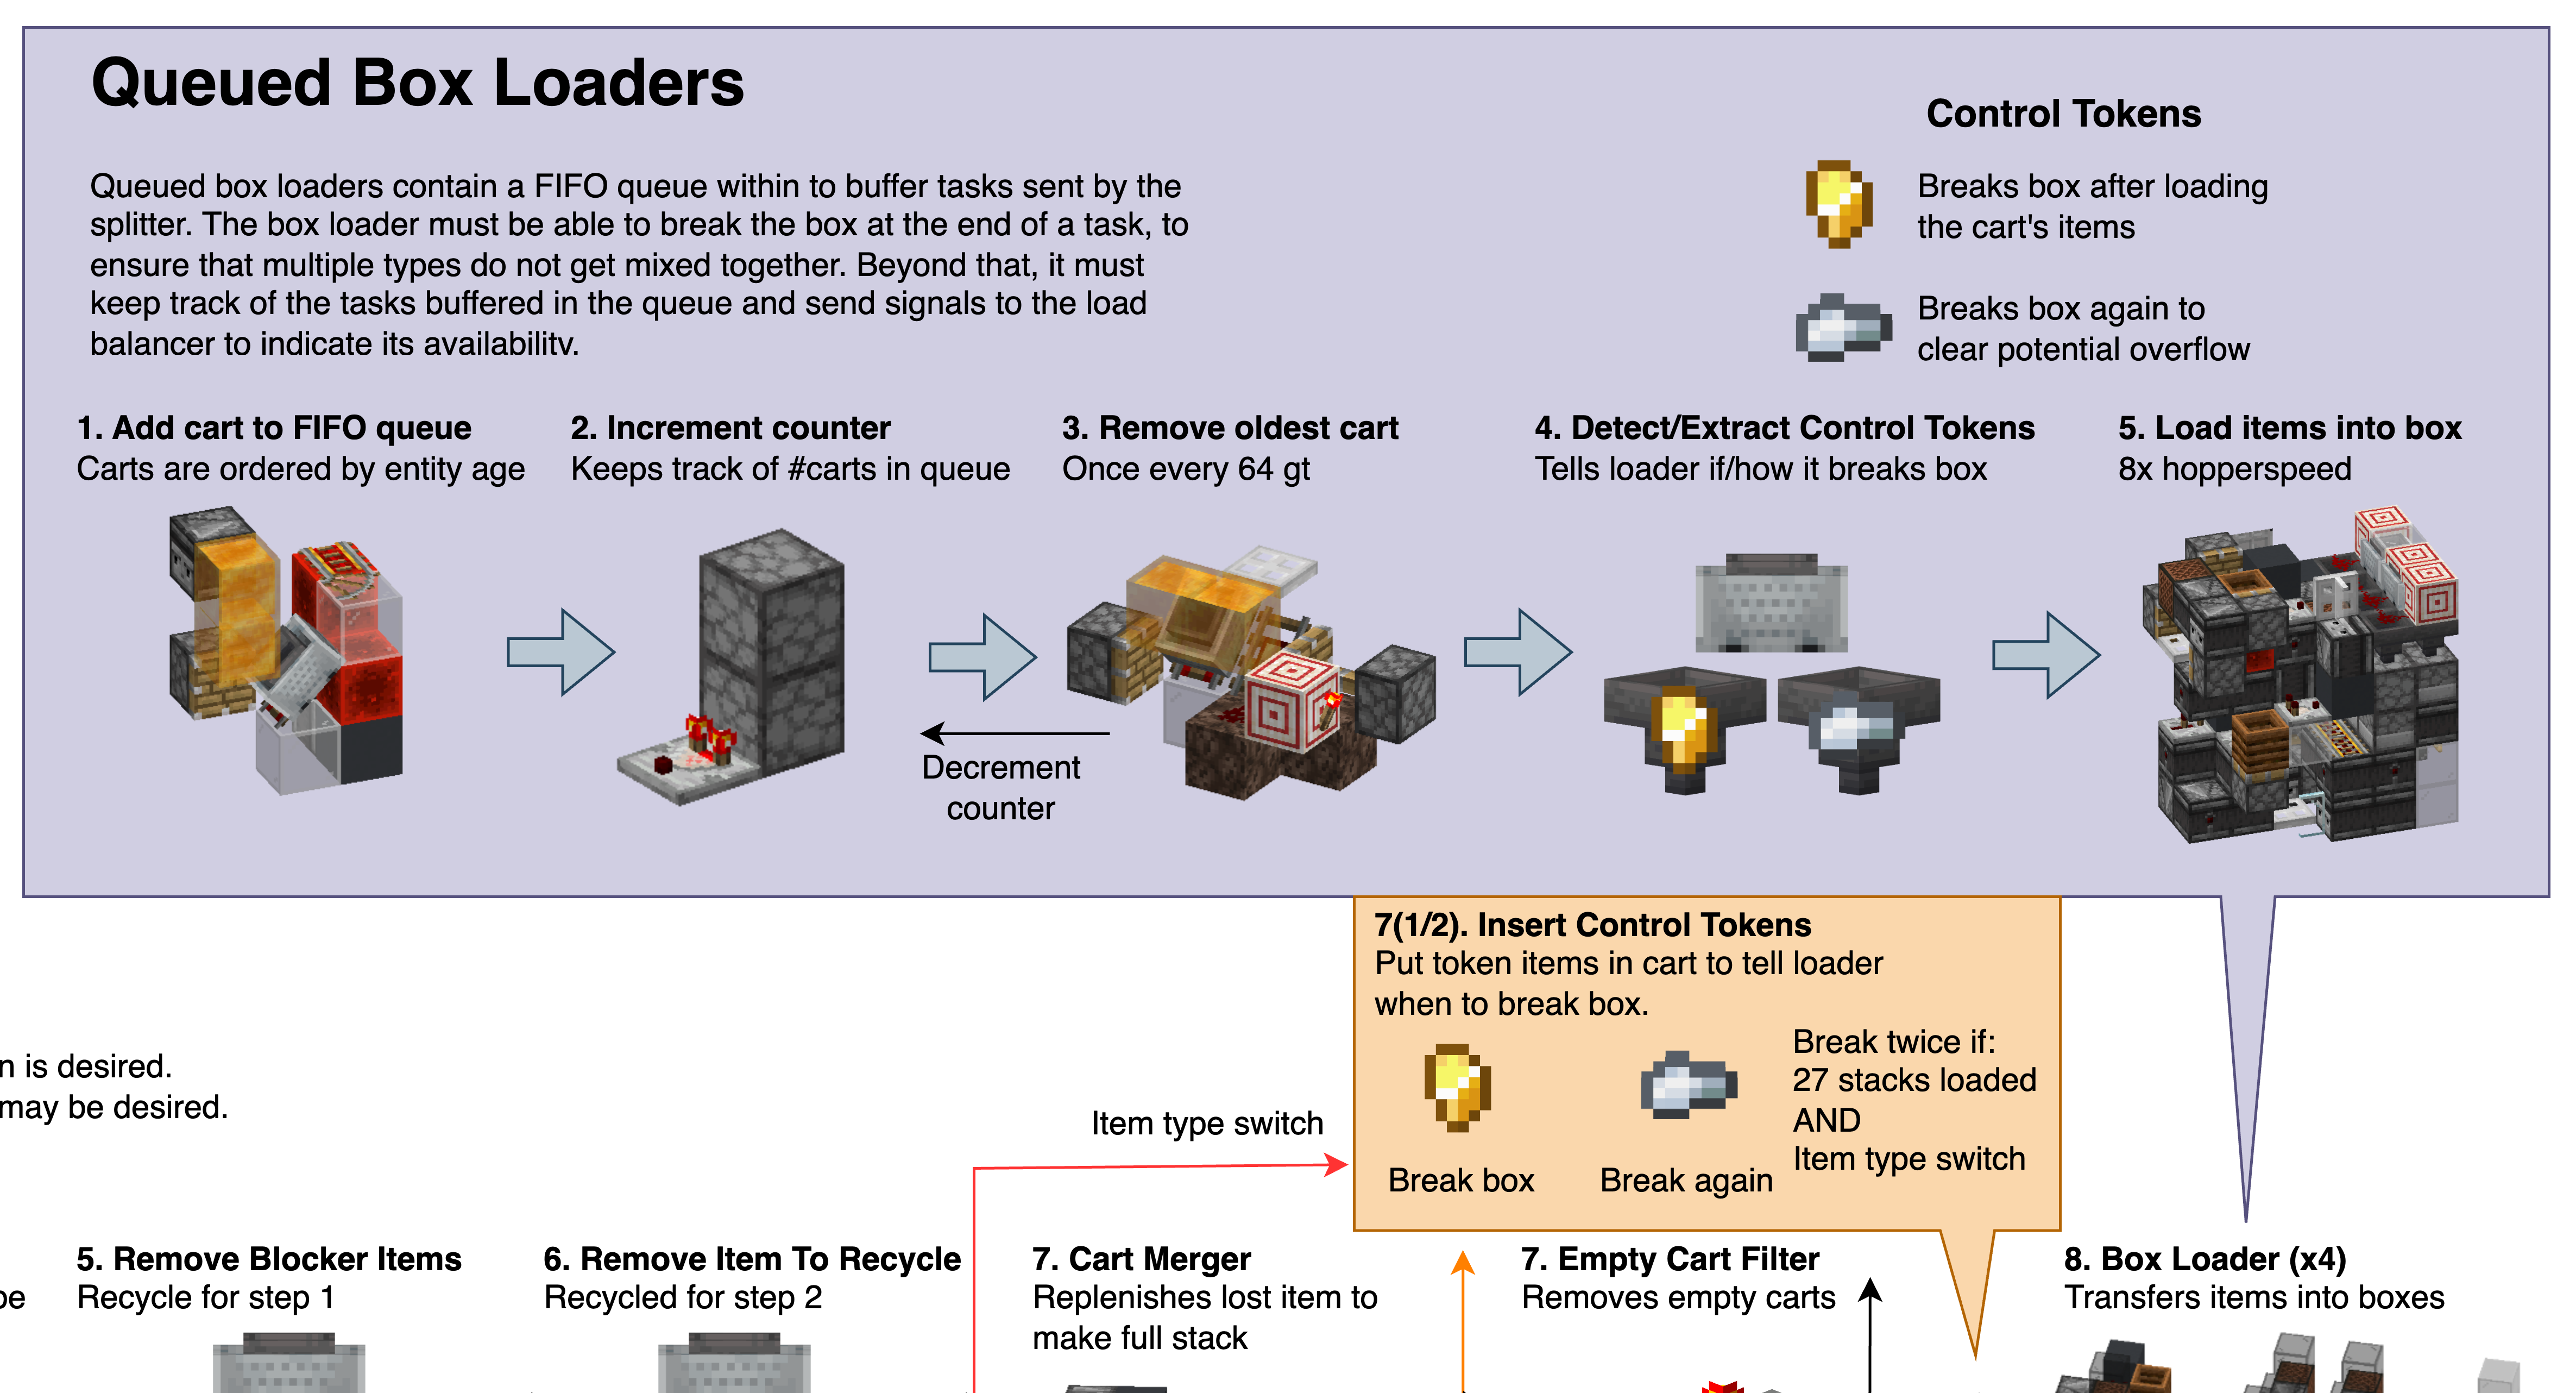
\includegraphics[width=0.85\paperwidth]{IdealSplitting3zoom.png}
\end{frame}
}

\begin{frame}
    \frametitle{3.3 Conclusion and Future Work}

    Conclusion:
    \begin{itemize}
        \item Queued loaders reduce number of loaders required
        \item Load balancing is important for good latency
        \item Reduced item entity movement for better performance
        \item Cart-based unloader and item refresher for box preservation
    \end{itemize}

    Future work:
    \begin{itemize}
        \item Improve wiring and compactness
        \item Micro-optimize device for reduced lag
    \end{itemize}

\end{frame}


\end{document}



